%%%%%%%%%%%%%%%%%%%%%%%%%%%%%%%%%%%%%%%%%%%%%%%%%%%%%%%%%%%%%%%%%%% 
%                                                                 %
%                            CHAPTER                              %
%                                                                 %
%%%%%%%%%%%%%%%%%%%%%%%%%%%%%%%%%%%%%%%%%%%%%%%%%%%%%%%%%%%%%%%%%%% 
\chapter{Results}
In this chapter, we will discuss the results of applying the OWL-ViT model to the shell dataset. We will first use the model as a zero-shot object detector. Secondly, we will use it as a N-shot object detector. For both, we will discuss the results for generic shell detection and detecting and classifying the shells. All PR-curve figures can be found in full size in Appendix \ref{app:pr_curves_full_size}.

\section{Zero-shot object detection}
For zero-shot object detection, we use the model with text embeddings. We also tried using negative queries, but this did not improve the results. For classless object detection, we added a few generic descriptions like 'seashell' and 'shell' to the queries.


% image with 2 subimages side by side (a) and (b)
\begin{figure}[h]
    \begin{adjustwidth}{-0.5in}{-0.5in}
        \centering
        \begin{subfigure}[b]{0.38\pdfpagewidth}
            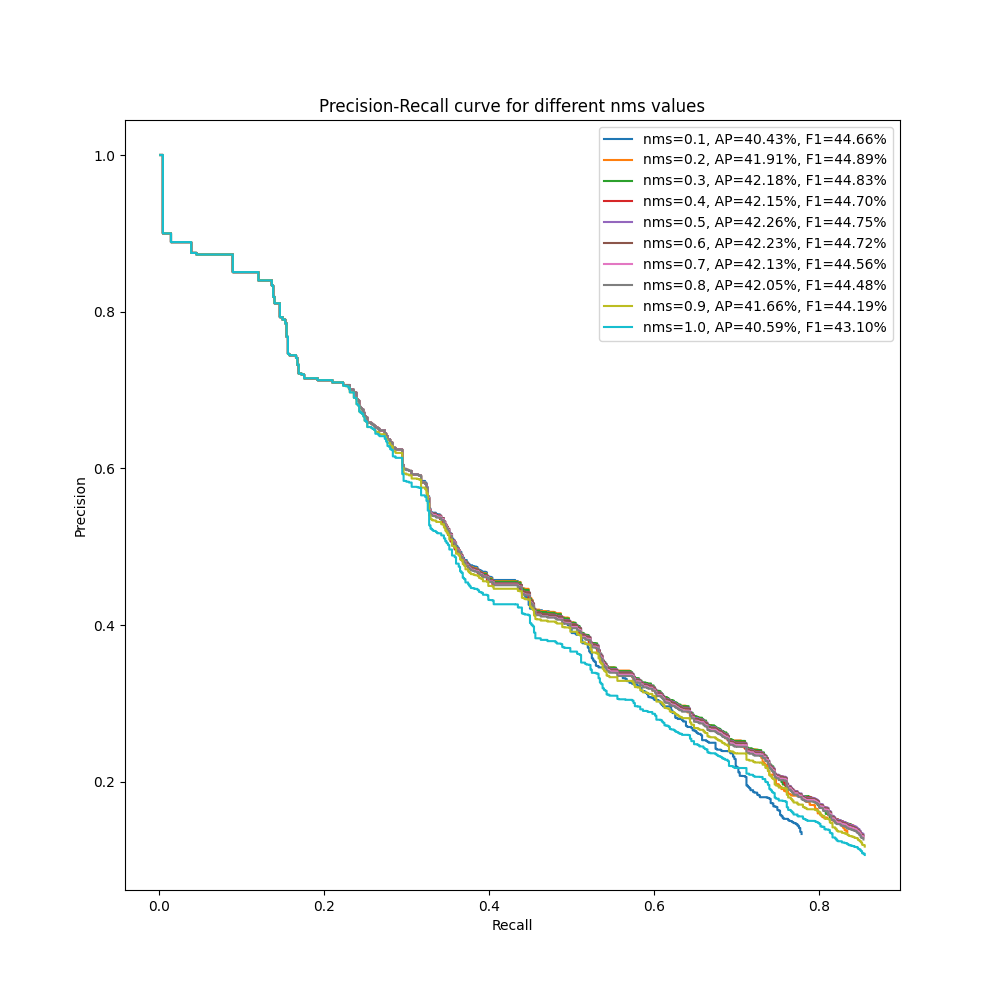
\includegraphics[width=\textwidth]{chapter5/text/classlessIoUPR.png}
            \caption{PR curve classless zero-shot object detection.}
            \label{fig:5_zero_shot_classless}
        \end{subfigure}
        \hfill
        \begin{subfigure}[b]{0.38\pdfpagewidth}
            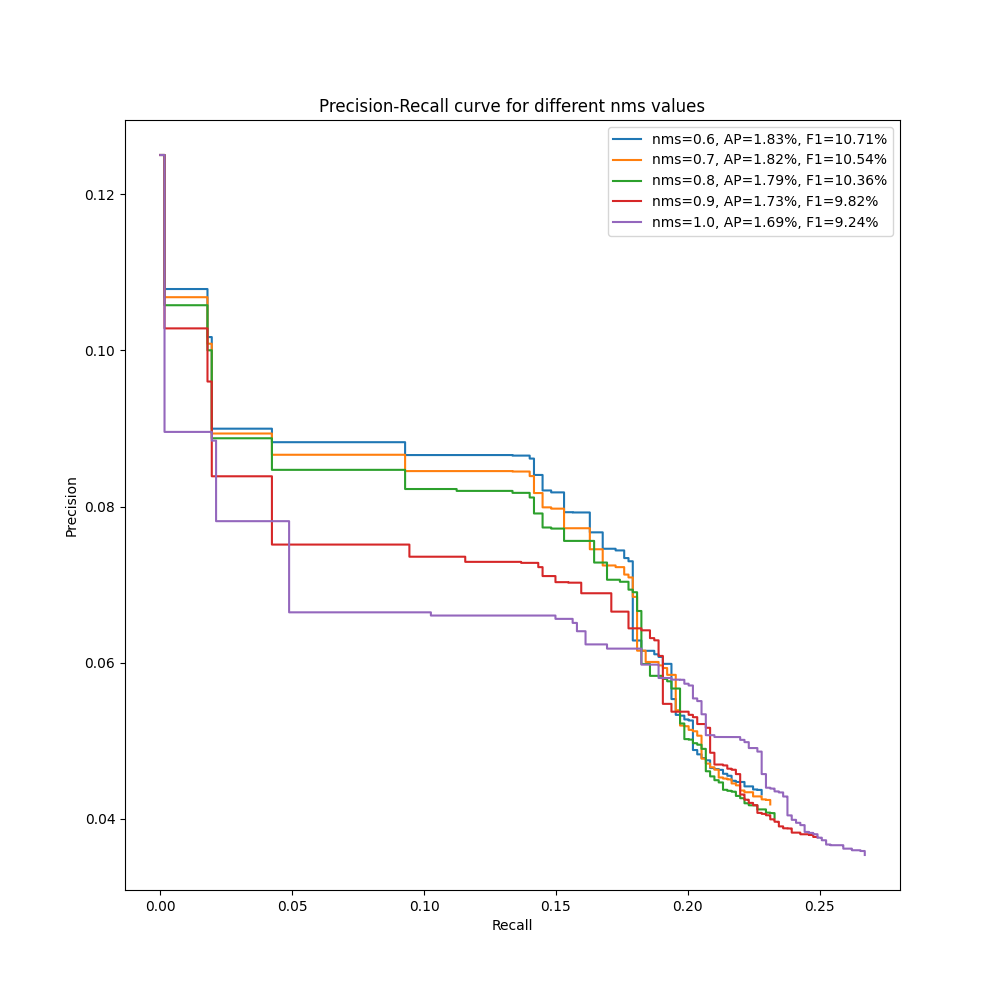
\includegraphics[width=\textwidth]{chapter5/text/classedIoUPR.png}
            \caption{PR curve classed zero-shot object detection.}
            \label{fig:5_zero_shot_classed}
        \end{subfigure}
    \end{adjustwidth}
    \caption{Zero-shot object detection.}
    \label{fig:5_zero_shot}
\end{figure}

For the classless detection, as seen in Fig \ref{fig:5_zero_shot_classed}, we obtain an AP of 42.26\% and an F1-score of 44.75\%. This seems like it could be used to generate proposals for manual classification. Upon visual inspection, however, we find very inconsistent results across images, as can be seen in Table \ref{fig:5_zero_shot_classless_examples}.

\begin{table}[h]
    % columns: threshold, image1, image2
    \centering
    \captionsetup{justification=centering}
    \begin{tabular}{|l|ll|}
        \hline
        Score & Image 1 & Image 2 \\ \hline
        0.1 & \includegraphics[width=0.4\textwidth]{chapter5/text/classless/0.1/1.jpg} & \includegraphics[width=0.4\textwidth]{chapter5/text/classless/0.1/3.jpg} \\ \hline
        0.2 & \includegraphics[width=0.4\textwidth]{chapter5/text/classless/0.2/1.jpg} & \includegraphics[width=0.4\textwidth]{chapter5/text/classless/0.2/3.jpg} \\ \hline
        0.3 & \includegraphics[width=0.4\textwidth]{chapter5/text/classless/0.3/1.jpg} & \includegraphics[width=0.4\textwidth]{chapter5/text/classless/0.3/3.jpg} \\ \hline
    \end{tabular}
    \caption{Examples of classless zero-shot object detection.}
    \label{fig:5_zero_shot_classless_examples}
\end{table}

For normal object detection, however, results aren't that great, with an mAP of 1.83\% and an F1-score of 10.71\%. When we look at the PR-curve for individual classes in Fig \ref{fig:5_zero_shot_classed_classes_PR} we find that some classes aren't even found at all.

\begin{figure}[h]
    \centering
    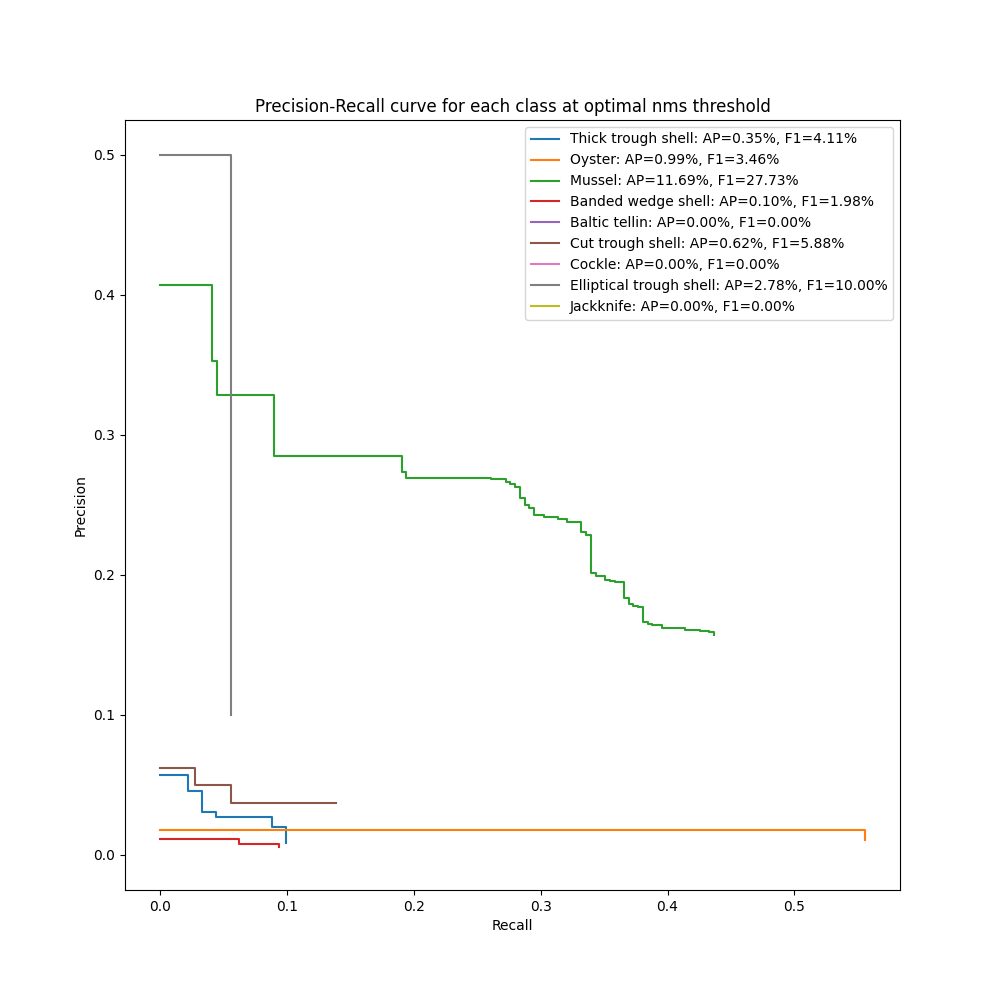
\includegraphics[width=0.7\textwidth]{chapter5/text/classesPR.png}
    \caption{PR curve for individual classes in zero-shot object detection.}
    \label{fig:5_zero_shot_classed_classes_PR}
\end{figure}

\section{N-shot object detection}
For N-shot object detection, we use the model with image embeddings. As the model now has visual examples of our objects, we expect better results than with zero-shot object detection. We will start by testing one-shot object detection, then we will test N-shot object detection with different values for N.

\subsection*{One-shot object detection}
One-shot object detection has always been quite a challenge, as it is difficult to learn a good representation of an object with only one example. As OWL-ViT is the SOTA model for this task, with some room to spare, we expect it to perform better than our zero-shot object detection. 

\begin{figure}[h]
    \begin{adjustwidth}{-0.5in}{-0.5in}
        \centering
        \begin{subfigure}[b]{0.4\pdfpagewidth}
            \includegraphics[width=\textwidth]{chapter5/img/classless\_1\_iouPR.png}
            \caption{PR curve classless.}
            \label{fig:5_n_shot_classless_pr_curve}
        \end{subfigure}
        \hfill
        \begin{subfigure}[b]{0.4\pdfpagewidth}
            \includegraphics[width=\textwidth]{chapter5/img/classed\_1\_iouPR.png}
            \caption{PR curve with classes.}
            \label{fig:5_n_shot_classed}
        \end{subfigure}
    \end{adjustwidth}
    \caption{1-shot object detection.}
    \label{fig:5_1_shot}
\end{figure}

For classless object detection, as seen in Fig \ref{fig:5_1_shot}, we obtain an AP of 40.89\% and an F1-score of 43.68\%. This is slightly worse than our zero-shot object detection. Upon visual inspection, we find that the model is more consistent in its detections, but still marks too many shards or parts of shells as detections, as can be seen in Table \ref{fig:5_n_shot_classless_examples}.

\begin{table}[H]
    % columns: threshold, image1, image2
    \centering
    \captionsetup{justification=centering}
    \begin{tabular}{|l|ll|}
        \hline
        Score & Image 1 & Image 2 \\ \hline
        0.7 & \includegraphics[width=0.35\textwidth]{chapter5/img/1_classless/0.7/1.jpg} & \includegraphics[width=0.35\textwidth]{chapter5/img/1_classless/0.7/2.jpg} \\ \hline
        0.8 & \includegraphics[width=0.35\textwidth]{chapter5/img/1_classless/0.8/1.jpg} & \includegraphics[width=0.35\textwidth]{chapter5/img/1_classless/0.8/2.jpg} \\ \hline
        0.9 & \includegraphics[width=0.35\textwidth]{chapter5/img/1_classless/0.9/1.jpg} & \includegraphics[width=0.35\textwidth]{chapter5/img/1_classless/0.9/2.jpg} \\ \hline
    \end{tabular}
    \caption{Examples of classless 1-shot object detection.}
    \label{fig:5_n_shot_classless_examples}
\end{table}

For normal object detection, however, results are better than with 0-shot, with an mAP of 5.46\% and an F1-score of 15.54\%. While this is still not great or useable, it is a significant improvement over 0-shot. When we look at the PR-curve for individual classes in Fig \ref{fig:5_n_shot_classed_classes_PR} we find a general improvement across the board.

\begin{figure}[H]
    \centering
    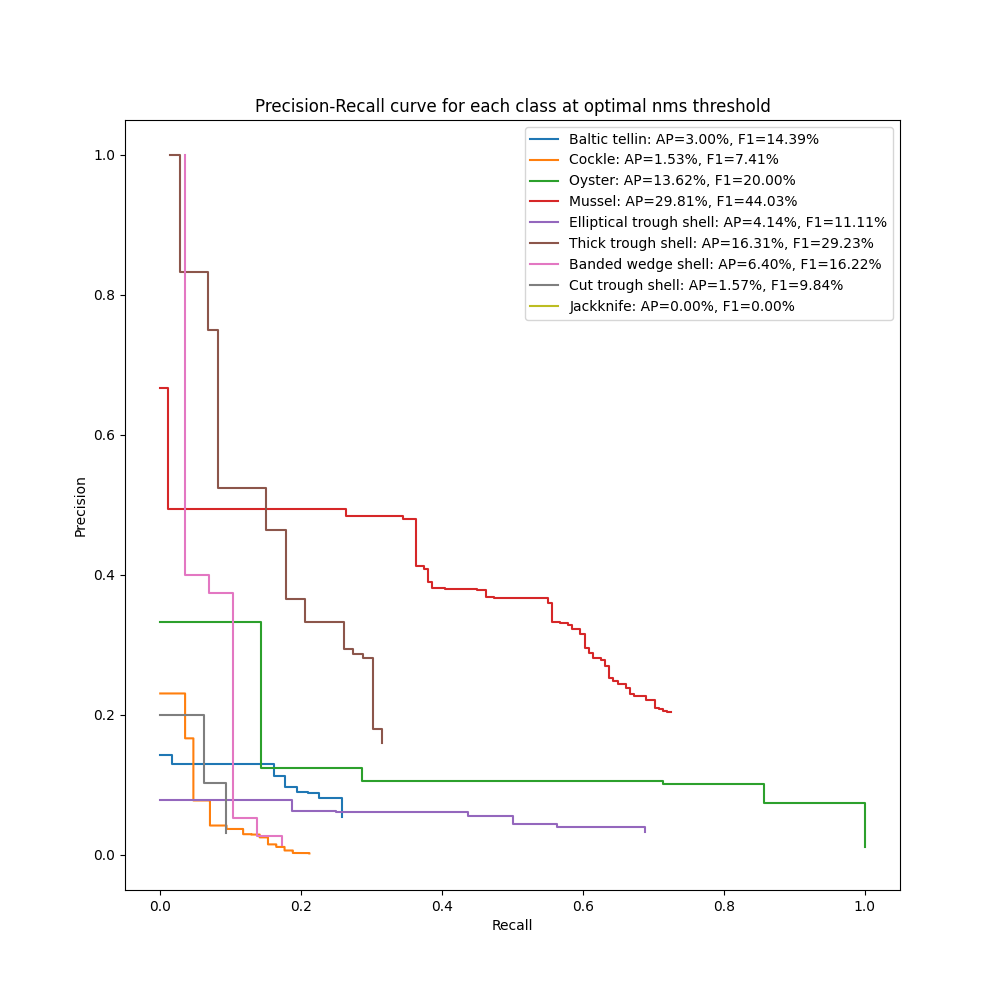
\includegraphics[width=0.7\textwidth]{chapter5/img/classed_1_classesPR.png}
    \caption{PR curve for individual classes in 1-shot object detection.}
    \label{fig:5_1_shot_classed_classes_PR}
\end{figure}

\subsection*{N-shot object detection}
Extracting multiple image embeddings and averaging those allows us to obtain more robust embeddings. This should reduce false detections and allow the model to better identify shells in difficult positions, like mostly buried or flipped shells. We will test this by using different values for N and comparing the results. The results can be found in Table \ref{tab:5_n_shot_results}. The PR curves for all N can be found in Appendix \ref{app:pr_curves_n_shot}. A visual comparison can be found in Table \ref{fig:5_n_shot_examples}.

\begin{table}[H]
    \centering
    \captionsetup{justification=centering}
    \begin{tabular}{|l|l|l|}
        \hline
        N & Classless AP & Classed mAP \\ \hline
        5 & 45.91 & 7.01 \\ \hline
        10 & 55.88 & 15.37 \\ \hline
        20 & 48.40 & 13.55 \\ \hline
        50 & 42.91 & 30.17 \\ \hline
    \end{tabular}
    \caption{Results for N-shot object detection.}
    \label{tab:5_n_shot_results}
\end{table}


\begin{table}[H]
    \begin{adjustwidth}{-0.5in}{-0.5in}
        % columns: N, image1, image2
        \centering
        \captionsetup{justification=centering}
        \begin{tabular}{|l|ll|}
            \hline
            N & Image 1 & Image 2 \\ \hline
            5 & \includegraphics[width=0.4\pdfpagewidth]{chapter5/img/5_classed/IMG20230217103106.jpg} & \includegraphics[width=0.4\pdfpagewidth]{chapter5/img/5_classed/IMG20230217104210.jpg} \\ \hline
            10 & \includegraphics[width=0.4\pdfpagewidth]{chapter5/img/10_classed/IMG20230217103106.jpg} & \includegraphics[width=0.4\pdfpagewidth]{chapter5/img/10_classed/IMG20230217104210.jpg} \\ \hline
            20 & \includegraphics[width=0.4\pdfpagewidth]{chapter5/img/20_classed/IMG20230217103106.jpg} & \includegraphics[width=0.4\pdfpagewidth]{chapter5/img/20_classed/IMG20230217104210.jpg} \\ \hline
        \end{tabular}
        \caption{Examples of classed N-shot object detection.}
        \label{fig:5_n_shot_examples}
    \end{adjustwidth}
\end{table}


We find a large peak in performance for 50-shot, important to consider though is that classes with fewer annotations than N are discarded. Looking at Fig \ref{fig:5_50_shot_classed_classes_PR} we see that we're only evaluating 4 classes. These classes also have the most unique features, which makes them easier to detect. The 50-shot results are thus not representative and should be discarded.

\begin{figure}[H]
    \centering
    \begin{adjustwidth}{-0.5in}{-0.5in}
        \begin{subfigure}[b]{0.4\pdfpagewidth}
            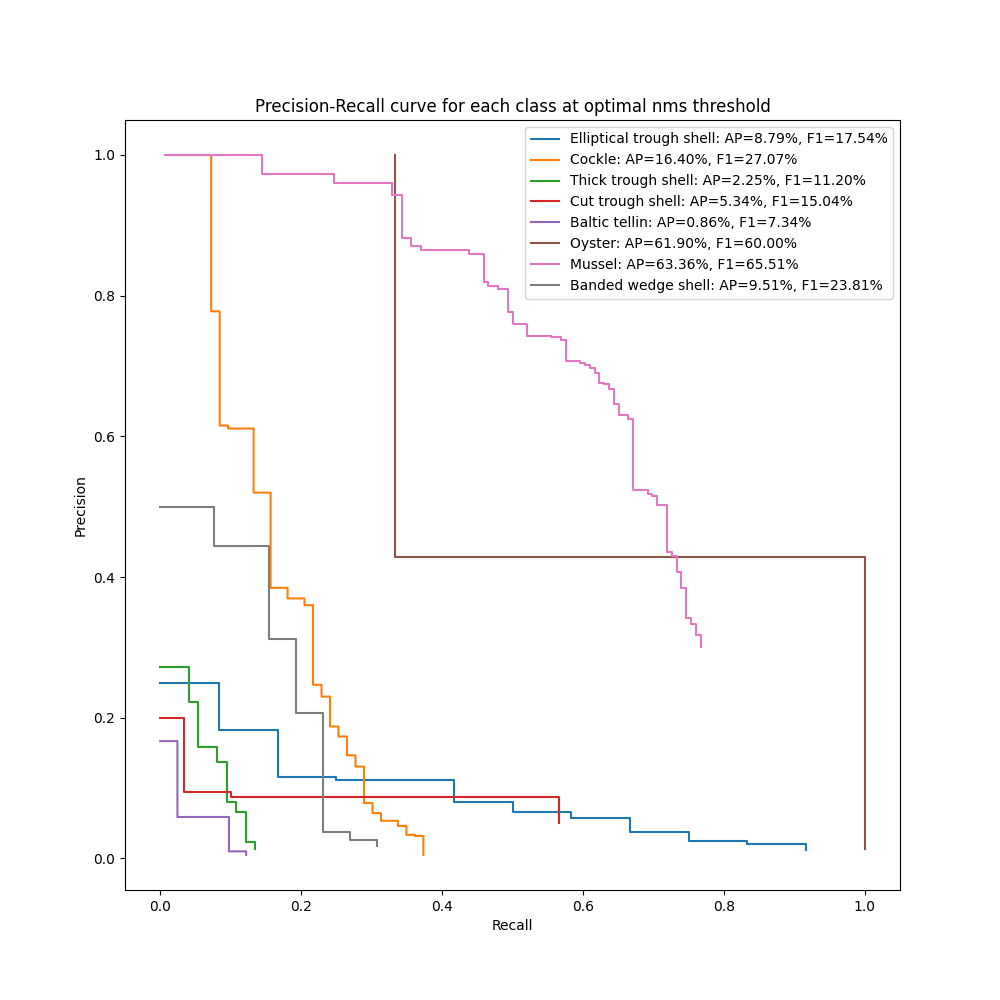
\includegraphics[width=\textwidth]{chapter5/img/classed_5_classesPR.png}
            \caption{PR curves for 5-shot object detection.}
            \label{fig:5_5_shot_classed_classes_PR}
        \end{subfigure}
        \hfill
        \begin{subfigure}[b]{0.4\pdfpagewidth}
            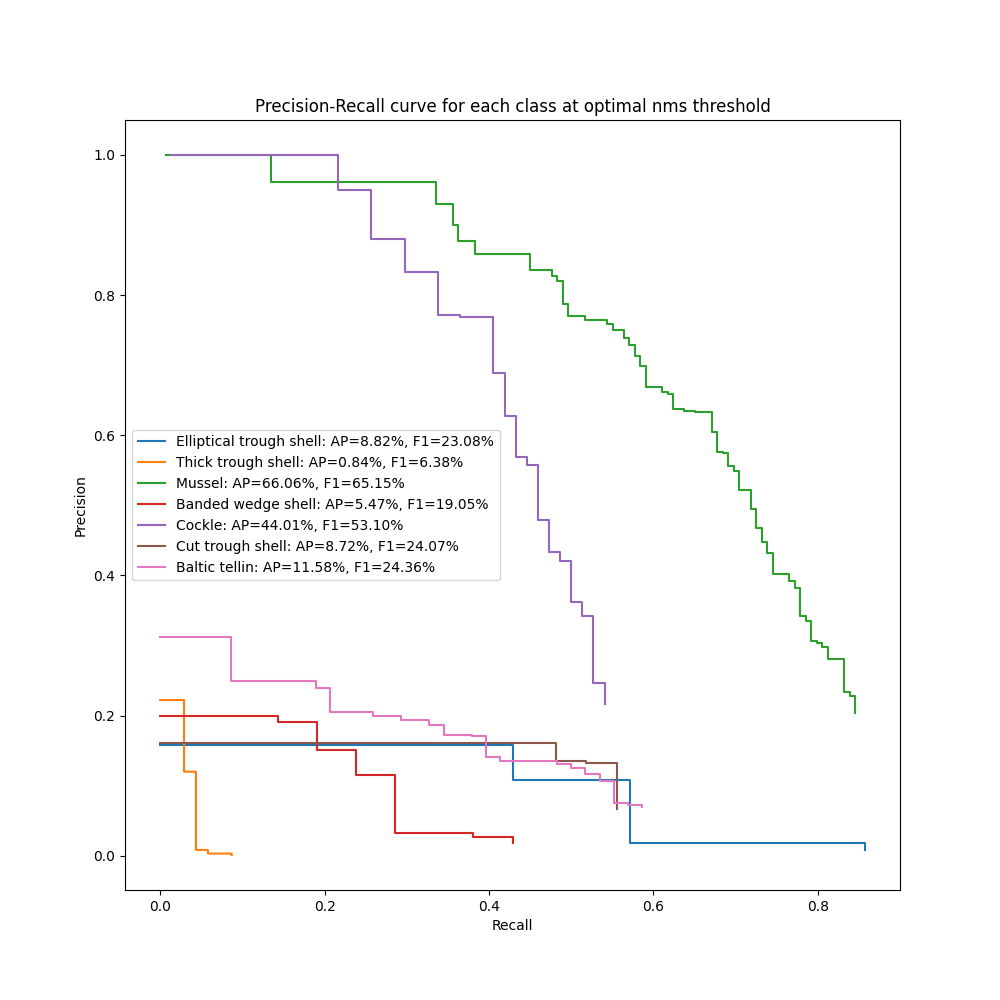
\includegraphics[width=\textwidth]{chapter5/img/classed_10_classesPR.png}
            \caption{PR curves for 10-shot object detection.}
            \label{fig:5_10_shot_classed_classes_PR}
        \end{subfigure}
        \begin{subfigure}[b]{0.4\pdfpagewidth}
            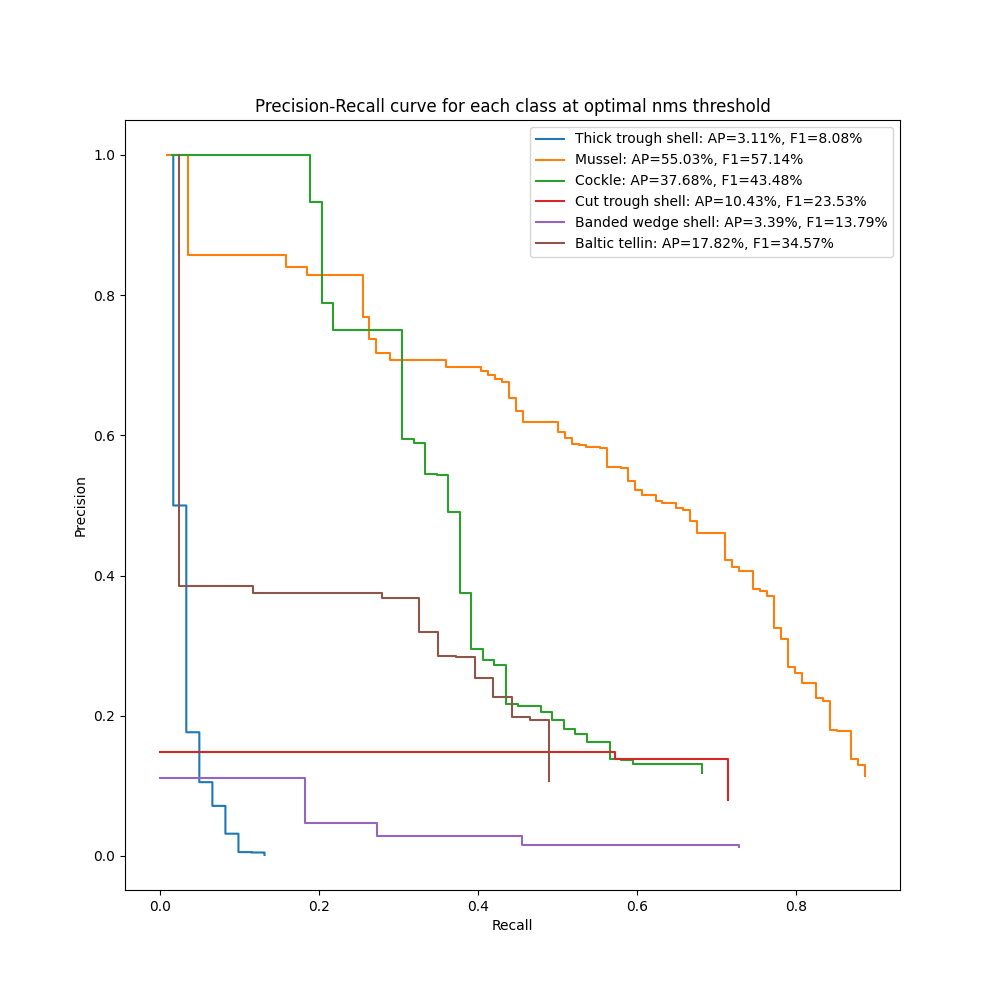
\includegraphics[width=\textwidth]{chapter5/img/classed_20_classesPR.png}
            \caption{PR curves for 20-shot object detection.}
            \label{fig:5_20_shot_classed_classes_PR}
        \end{subfigure}
        \hfill
        \begin{subfigure}[b]{0.4\pdfpagewidth}
            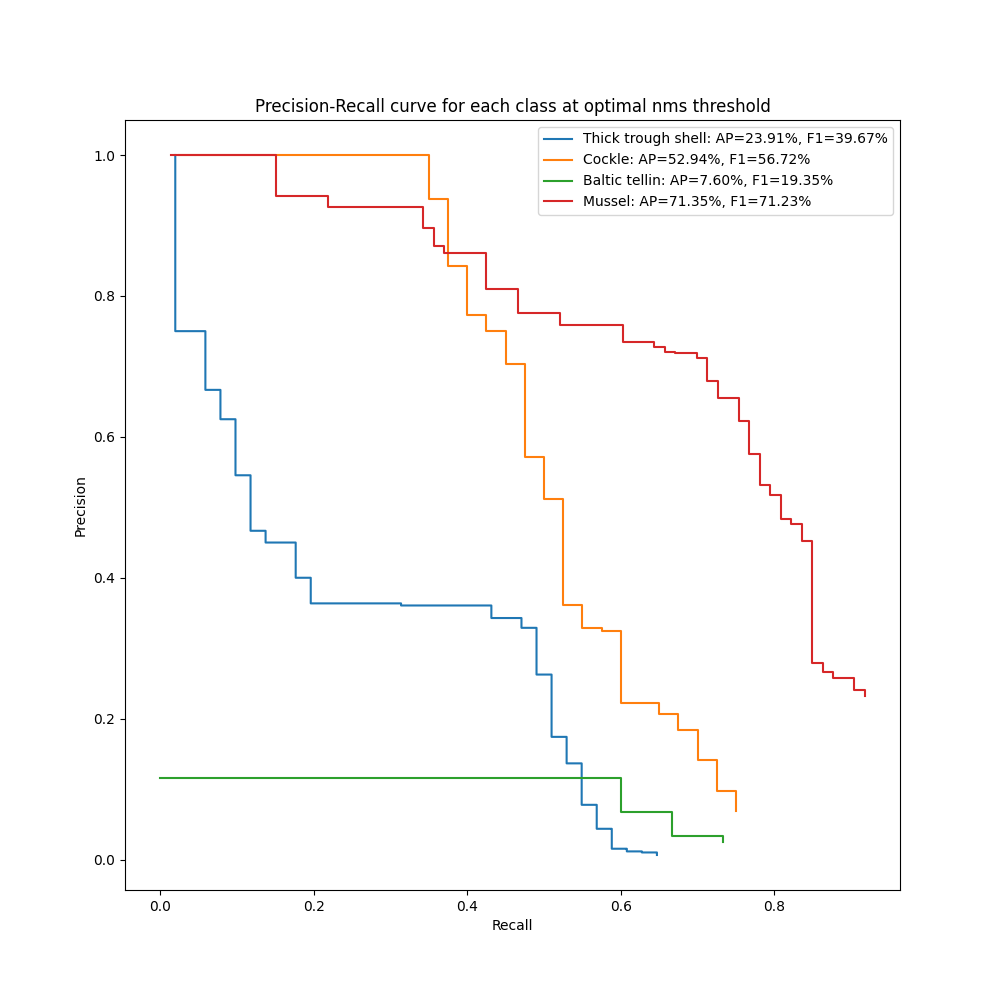
\includegraphics[width=\textwidth]{chapter5/img/classed_50_classesPR.png}
            \caption{PR curves for 50-shot object detection.}
            \label{fig:5_50_shot_classed_classes_PR}
        \end{subfigure}
        \caption{PR curves for individual classes in N-shot object detection.}
        \label{fig:5_n_shot_classed_classes_PR}
    \end{adjustwidth}
\end{figure}

\section{Using all embeddings}
As mentioned before in Section \ref{sec:3_notebook_implementation} we currently throw away a lot of generated embeddings as they go over the N-amount of N-shot. Using these could on the other hand be compared to a train-test split (no validation set is required as we're not training). For our most common type of shells, this could bring a major improvement to the robustness of the embeddings. The results for this can be found in Table \ref{tab:5_all_embeddings_results}, here N is the minimum number of embeddings for a class instead of an exact amount of embeddings per class. The highest impact is, as expected since the base robustness is lower, on the lower values for N. For certain options, we do see a slight degradation in performance, but overall the results are slightly better than with the exact N-shot.

\begin{table}[H]
    \centering
    \captionsetup{justification=centering}
    \begin{tabular}{|l|l|l|}
        \hline
        N & Classless AP (strict N) & Classed mAP (strict N) \\ \hline
        1 & 55.05 (40.89) & 14.61 (5.46) \\ \hline
        5 & 56.18 (45.91) & 13.36 (7.01) \\ \hline
        10 & 57.90 (55.88) & 14.30 (15.37) \\ \hline
        20 & 51.45 (48.40) & 17.20 (13.55) \\ \hline
        50 & 42.45 (42.91) & 27.83 (30.17) \\ \hline
    \end{tabular}
    \caption{Results for N-shot object detection using all embeddings.}
    \label{tab:5_all_embeddings_results}
\end{table}

\section{Discussion}
Visually inspecting our results we find some reasons for the mediocre results, like false positives and wrong detections.

\subsection*{False positives}
The model finds many shells in places without annotations. These detections range from rocks to unidentifiable fragments to broken shells to shells we missed during annotating. Most false positives at high confidence are of the last two types. Solving this would have little to do with our implementation, but rather with the dataset. Annotating the dataset better is easier said than done, as not every shell is easy to annotate. We will go into more detail on this in the next section.

\subsection*{Dataset quality}
Annotating the shell dataset isn't easy. We are not experts who can see the minute details that differentiate two similar shells, like the 'cut trough shell' and the 'thick trough shell' as shown in Fig \ref{fig:5_wikipedia_cut_vs_thick}. We also have to deal with shells that are mostly buried or broken, how broken should a shell be but still be annotated? Some shells, like the cockle, have a very recognizable pattern even in fragments. Expanding the dataset would also possibly make other methods possible besides few-shot object detection or it would at least give us more robust results.


\begin{figure}[H]
    \centering
    \begin{subfigure}[b]{\textwidth}
        \includegraphics[width=\textwidth]{chapter5/wikipedia\_cut\_trough\_shell\_small.jpg}
        \caption{The cut trough shell.}
        \label{fig:5_wikipedia_cut_trough_shell}
    \end{subfigure}
    \hfill
    \begin{subfigure}[b]{\textwidth}
        \includegraphics[width=\textwidth]{chapter5/wikipedia\_thick\_trough\_shell\_small.jpg}
        \caption{The thick trough shell.}
        \label{fig:5_wikipedia_thick_trough_shell}
    \end{subfigure}
    \caption{The cut trough shell and the thick trough shell. Images from Wikipedia.}
    \label{fig:5_wikipedia_cut_vs_thick}
\end{figure}

